

\documentclass[a4paper,11pt,twocolumn]{article}
	
	\usepackage{geometry}
	\geometry{hmargin=2cm,vmargin=2cm}
	
	\usepackage{algorithm2e}
	\usepackage{graphicx}
	\usepackage{tabularx}
	\usepackage{fourier}
	\usepackage{hyperref}
	\usepackage{multirow}
	\usepackage{caption}
	\usepackage{subcaption}
	\usepackage{amsmath}
	\usepackage{float}
	
	\usepackage{xcolor}
	\usepackage{listings}
	
	\definecolor{mGreen}{rgb}{0,0.6,0}
	\definecolor{mGray}{rgb}{0.5,0.5,0.5}
	\definecolor{mPurple}{rgb}{0.58,0,0.82}
	\definecolor{backgroundColour}{rgb}{0.95,0.95,0.92}
	
	\lstdefinestyle{CStyle}{
		backgroundcolor=\color{backgroundColour},   
		commentstyle=\color{mGreen},
		keywordstyle=\color{magenta},
		numberstyle=\tiny\color{mGray},
		stringstyle=\color{mPurple},
		basicstyle=\footnotesize,
		breakatwhitespace=false,         
		breaklines=true,                 
		captionpos=b,                    
		keepspaces=true,                 
		numbers=left,                    
		numbersep=5pt,                  
		showspaces=false,                
		showstringspaces=false,
		showtabs=false,                  
		tabsize=2,
		language=C
	}
	
	\author{
		Alexane Boldo\\
		Intern\\
		ENS Rennes
	}
	
	\title{Side-channel attacks on Ascon to find the location of the leakage}
	\date{}
	
	%\counterwithout{section}{chapter}
	%\counterwithout{figure}{chapter}
	
	\begin{document}
		\maketitle
		
		% Un petit résumé
		\begin{abstract}
			This article finds a new side-channel attack (SCA) on the Nationale Institute of Standards and Technology (NIST) winner Ascon using observations on the S-box equations to link output and key and attacks the decryption process. It also analyses where exactly the leak occurs in the S-box to try to find the cause for the leak to better mask the power consumption.
		\end{abstract}
		
		%\tableofcontents
		
		\section{Introduction}
		Though mathematically secure, cryptographic algorithms can still be broken. Indeed leakages happen during the computation of the encryption, which can be observed and analysed to figure out the key. Such leakages can be the computation time, the power consumption or the electromagnetic radiations and can lead to attacks recovering the key, called side-channel attacks (SCA). Therefore a whole field of cybersecurity consists of analysing which computations leak the most data.\\
		This article will focuse on Ascon \cite{ascon}, the winner of the Nationale Institute of Standards and Technology (NIST) competition for Authenticated Encryption with Associated Data (AEAD), which became the standard for lightweight cryptography \cite{norme}. Multiple attacks \cite{cpa_lin,dl_cpa} based on Correlation Power Analysis (CPA) have already been performed and analysed \cite{cpa_analysis} to find a stronger implementation of Ascon, using masking to render SCA harder.\\
		In the following, CPA will be used to determine where exactly the leakage is the clearer, by analysing the output of the S-box in the permutation and we will deduce a new attack from the analysis by Sarry \cite{these} using the equations of the permutation to attack the output of the substitution layer of the first-round of the permutation.
		
		\section{Description of Ascon}
		This paper will focus on the AEAD Ascon as described in the norm \cite{norme}. This paper will especially focuse on the decryption phase to use the leaks in order to recover the key.
		
		\begin{algorithm}[h]
			\KwData{128-bit key $K$ and nonce $N$, associated data $A$, ciphertext $C$ and 128-bit tag $T$}
			\KwResult{checks authentication with $T$, if it is returns plaintext $P$ otherwise returns fail}
		\end{algorithm}
		
		This algorithm uses a 320-bit state, divided into 5 64-bit words and modified through 4 phases : the initialization, the associated data process, the ciphertext process and the finalization. IV is a known constant given in the norm \cite{norme}, and in the following this paper will refer to the rate as $r=128$, the number of rounds a as $a=12$ and the number of rounds b as $b=8$.
		
				
		This decryption uses a permutation $p = p_L \circ p_S \circ p_C$ which is used at all phases of the decryption and will be the target of the attack. This permutation is itself divided into three layers, the constant-addition layer $p_C$ that adds to the end of the third word an 8-bit round-dependent constant, the substitution layer $p_S$ which is a 5-bit S-box taking the $j^{th}$ bit of each word, and the linear-diffusion layer $p_L$ rotating each word. Each step \ref{perm} and each notation \ref{notations} is described in more details in the annex.
		
		\begin{figure}[h]
			\centering
			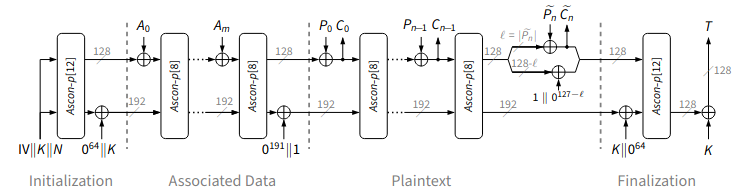
\includegraphics[width=0.5\textwidth]{encryption}
			\caption{Ascon Encryption process from \cite{norme}}
			\label{fig:enc}
		\end{figure}
		
		\begin{enumerate}
		\item Initialization: state creation and modification
		$$S \leftarrow p^{a}( \underbrace{IV}_{S_0}||\underbrace{K}_{S_1,S_2}||\underbrace{n}_{S_3,S_4})$$
		$$S \leftarrow S \oplus 0^{192} || K$$
		\item Associated data process: updates the state using blocks of $r$-bits form $A=(A_1||..||A_s)$
		$$\forall i \in \llbracket 1,s \rrbracket,\  S \leftarrow p^b((S_{<=r} \oplus A_i)||S_{>r})$$
		then the least-significant bit is flipped
		\item Ciphertext process: $C = (C_1 || ... || C_t)$ with $C_i$ of size $r$ and $l=|C| \% r$. Each block of the ciphertext is then computed:
		$$P_i \leftarrow S_{<=r} \oplus C_i$$
		$$S \leftarrow \left \{	\begin{array}{ll}
			p^b(C_i||S_{>r}) & if\ 1 \le i < t \\
			C_i||S_{>r} \oplus  (0^{l-1}||1||0^{320-1-l}) & if\ 1 \le i = t
		\end{array}
		\right.$$
		\item Finalization: computes the tag thanks to the key and the state
		$$S \leftarrow p^a(S \oplus (0^{64} || K || 0^{256-|K|}))$$
		$$T' \leftarrow S_{r\ last\ bits} \oplus K$$
		if $T'= T$, returns $P = P_1 || ... || P_t$, otherwise returns \verb|fail|
		\end{enumerate}
		
		\section{Methodology}
		We implemented our version of Ascon, given in this repository\footnote{\url{https://github.com}} to visualize the possible implementation weaknesses, which we compared to the reference implementation\footnote{\url{https://github.com/ascon/ascon-c/blob/main/crypto\_aead/asconaead128/ref}} from the authors of Ascon \cite{ascon}.
				
		Our version has the advantage to be able to follow other constants than those given by the norm. The values defined have to follow the following restrictions:
		
		\begin{center}
			\footnotesize
			\begin{tabular}{|c|c|}
				\hline
				\textbf{Variable} & \textbf{Definition domain}\\
				\hline
				\verb|KEY_LENGTH| & $\in 8\mathbb{N} \bigcap \llbracket 1,320 \rrbracket$\\
				\hline
				\verb|TAG_LENGTH| & $\in 8\mathbb{N} \bigcap \llbracket 1,\verb|KEY_LENGTH| \rrbracket$\\
				\hline
				\verb|RATE| & $\in 64\mathbb{N} \bigcap \llbracket 1,320-\verb|KEY_LENGTH| \rrbracket$\\
				\hline
				\verb|NB_ROUNDS_A| & \multirow{2}{*}{$\in \llbracket 1,16 \rrbracket^2$}\\
				\verb|NB_ROUNDS_B| &\\
				\hline
				\verb|VERSION| & $=1$ \\
				\hline
			\end{tabular}
		\end{center}
		
		In order to attack the implementations, a ChipWhisperer-Lite board with an XMEGA target microcontroller (CW1173) is used to capture the power consumption during the execution of the encryption, as it gives clearer traces than in real-life scenarios.
		
		\begin{figure}[h]
			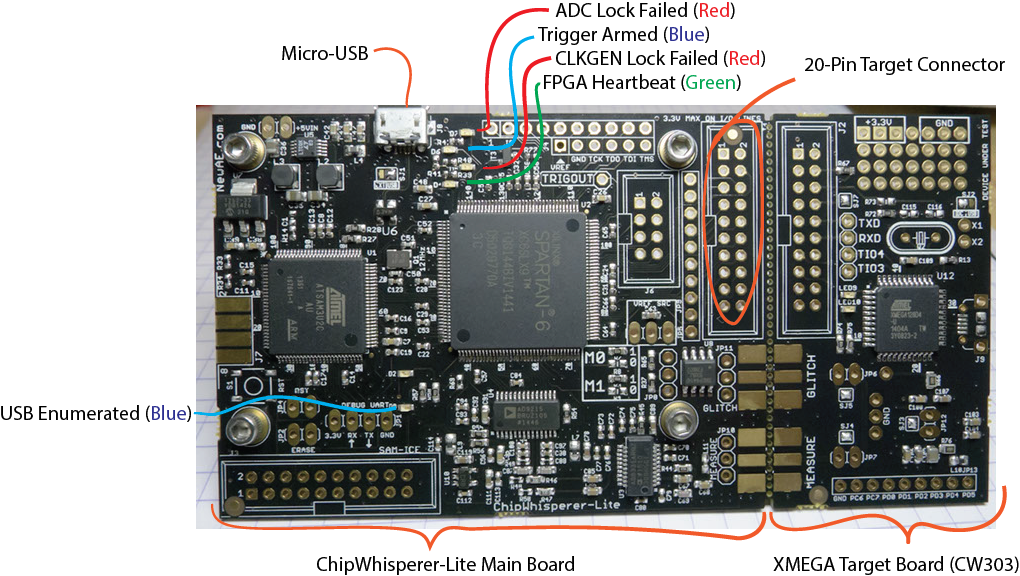
\includegraphics[width=0.5\textwidth]{cwlite_basic1}
			\caption{ChipWhisperer from \cite{cwdoc}}
			\label{fig:cw}
		\end{figure}
		
		To facilitate the capture, triggers were added in the first round of the permutation, during the initialization stage, in order to start the recording of the power consumption.
		
		40K traces with a fixed key and variable nonces during the $p_S$ layer, 10K traces with variable keys and nonces during the $p_S$ layer, 10K traces with variable keys and a fixed nonce during the $p_S$ layer, and 50K traces with a fixed key and variable nonces during the $p_L$ were recorded on both the reference implementation and our own. The following section will explain why this choices were made.
		
		\section{Observations for CPA attacks}
		\subsection{Correlation Power Analysis (CPA) definition}
		Correlation Power Analysis is a type of attack using the recording of multiple traces of the execution of a known cryptographic algorithm to recover the private key. It can be blind (the attacker doesn't know neither the plaintext nor the ciphertext) or not. It is often based on the divide-and-conquer approach where the attacker recovers the key portion-by-portion (often byte-by-byte or bit-by-bit). The following explaination will take the notations used in the course \cite{cours}.
		
		\begin{enumerate}
			\item \textbf{Campagne:}
			\begin{itemize}
				\item Let's first define the target $k$ that will take all its possible values (e.g. for one byte of the key, its 256 values)
				\item Then the first step is to compute multiple traces of the targeted algorithm to gain observables (e.g. the plaintext and the power consumption as a function of time)
				\item Find an attack path, i.e. a relation between observables and the target: $\mathcal{R}(k,O_S) = O_R$. This depends on physical functions, called leak functions, and cannot be computed
			\end{itemize}
			\item \textbf{Prediction:} Because the exact leak functions cannot be computed, the attacker has to find a model to approximate it (e.g. the Hamming Weight (HW) of the byte for the power consumption, as the consumption of writing in a register depends on whether it is a 1 or a 0 that is written), it gives a new relation model, called a theoritical attack path: $\mathcal{R}_m(k,O_S) = P_{m,k}$
			\item \textbf{Confrontation:} The attacker has to find a distinguisher, a statistical function that will put an hypothesis $k_d$ upfront of the others by confroning $O_R$ and $P_{m,k}$ (e.g. the Pearson correlation between the vector of HW and the consumption at each timestamp $t$). This also gives points of interest, i.e. timestamps where the target is used.
		\end{enumerate}

		This attack is well established on the previous encryption standard AES \cite{aes,cpa_aes} by attacking the S-box, however in Ascon the S-box is computed vertically and not horizontally, whereas the results are written in the words, therefore horizontally.
		
		\begin{figure}[h]
			\centering
			\begin{subfigure}{.18\textwidth}
				\centering
				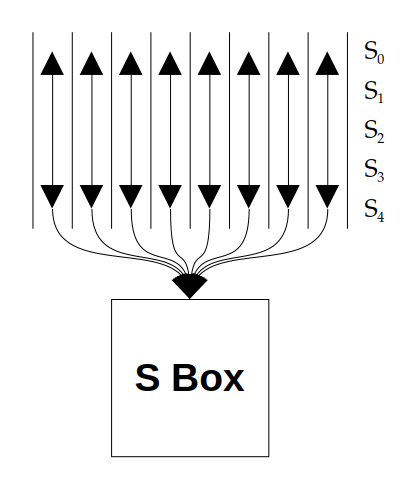
\includegraphics[width=1\linewidth]{sbox_computation}
				\caption{Computing}
				\label{fig:comp}
			\end{subfigure}
			\begin{subfigure}{.22\textwidth}
				\centering
				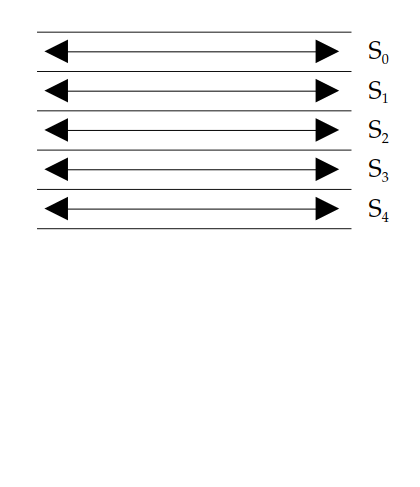
\includegraphics[width=.8\linewidth]{sbox_writing}
				\caption{Writing in the register}
				\label{fig:writ}
			\end{subfigure}
			\caption{Comparison of the direction for computing the S-box and writing in the register for the first byte of the five words}
			\label{fig:direction}
		\end{figure}
		
		Therefore it is pertinent to wonder, like Sarry in \cite{these}, whether the leak is horizontal or vertical, in order to determine if the S-box leaks because of the computation or of the writing in the register and to find better strategies of masking. Later, this article will refer to attacks on one byte of the last word of the state as horizontal attacks and to the ones on the concatenation of the 5 bits at position $j$ on each word of the state as vertical attacks.
		
		\subsection{Choosing a theoritical attack path and a distinguisher} \label{choice}
		\subsubsection{Horizontal attack on the S-box}
		In this part, the traces used are those mesuring during the computation of the S-box on our implementation, with variable keys and a fixed nonce, in order to see what functions show the most influence from the key.
		
		The goal is to see if there is an adequate distinguisher for the key hypothesis, using the HW of the first horizontal byte. Two statistical functions seem promising: the Pearson correlation usually used in CPA attacks, which failed to conclude for more than 40K traces in \cite{dl_cpa} and the mutual information.
		
		\begin{figure}[h]
		\centering
		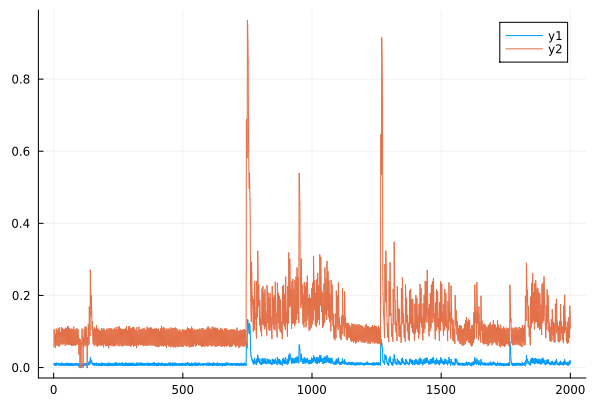
\includegraphics[scale=0.3]{horizontal_one_byte}
		\caption{Graph of the mutual information between the power consumption and the Hamming weight of the first byte of $S_4$ in blue and its value in orange, as a function of time}
		\label{hHW&val}
		\end{figure}
		
		In the graph \ref{hHW&val}, there are multiple points of interest that seem to show an influence from the key on the power consumption on a few instances, which is a good sign to be able to find the key later. To visualise how the points of interest for each byte correlate, the graph \ref{hHW8_zoom} shows that the use of each byte of key is successive, which is logical. 
		
		\begin{figure}[h]
			\centering
			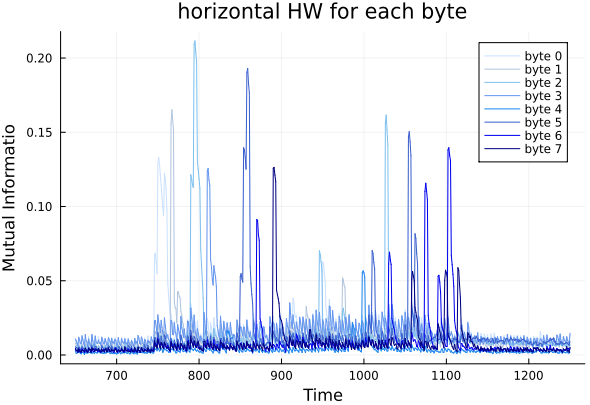
\includegraphics[scale=0.3]{hHW_8_bytes_zoom}
			\caption{Mutual information between power consumption and Hamming weight of each of the 8 bytes as functions of time}
			\label{hHW8_zoom}
		\end{figure}

		\begin{figure}[h]
			\centering
			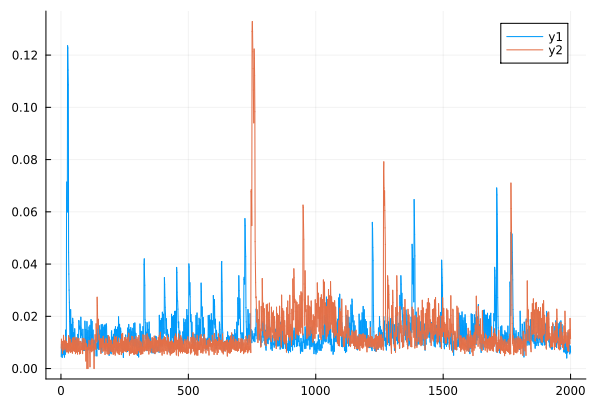
\includegraphics[scale=0.3]{comp_ref_hHW}
			\caption{Mutual information between power consumption and horizontal Hamming Weight on the reference implementation in blue and on our own in orange}
			\label{compref}
		\end{figure}
		
		To check if our implementation is worse than the reference one, the graph \ref{compref} is useful and shows that both of them have clear leaks however, these leaks don't happen at the same time, since the S-box is not written exactly the same. 
		
		\begin{figure}[H]
			\centering
			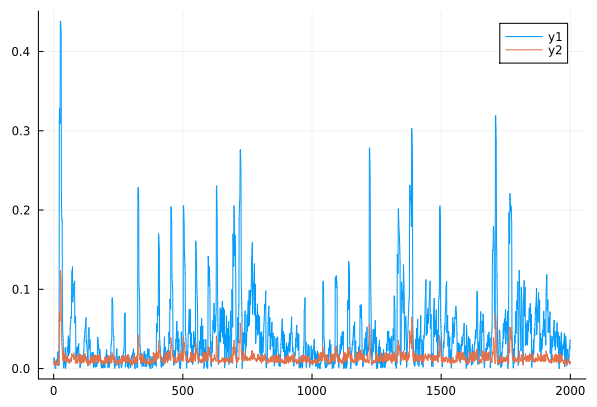
\includegraphics[scale=0.3]{corr_vs_MI_hHW}
			\caption{Mutual information (in orange) and absolute Pearson correlation (in blue) for a horizontal attack on the reference implementation}
			\label{corvsMI}
		\end{figure}
		
		Let's now compare the mutual information with the Pearson correlation. In the graph \ref{corvsMI}, a reassuring observation is that points of interest are the same no matter the distinguisher.Furthermore, though the absolute value is greater for the Pearson correlation, points of interest appear clearer after normalisation with the mutual iformation, which can help on the attack.
		
		\subsubsection{Vertical attack on the S-box}
		First, let's use the same traces as before and compare to see if there is an adequate distinguisher using the HW of the first output of the S-box.
		
		\begin{figure}[h]
			\centering
			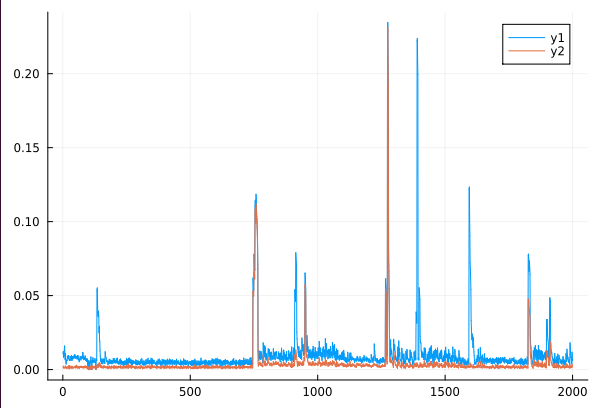
\includegraphics[scale=0.3]{vertical_one_bit}
			\caption{Mutal information between power consumption and Hamming weight of the concatenation of the first bit of each of the word of $S$ in orange and its value in blue}
			\label{vHW}
		\end{figure}
		
		\begin{figure}[h]
			\centering
			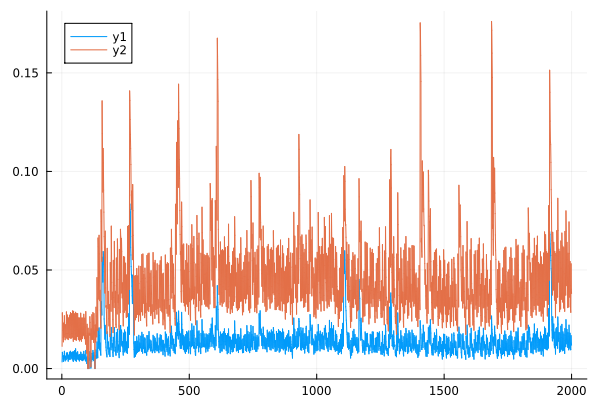
\includegraphics[scale=0.3]{vertical_one_byte}
			\caption{Same thing as \ref{vHW} but for random nonces ith Hamming weight in blue and value in orange}
			\label{vHW&val}
		\end{figure}
		
		From the graph \ref{vHW}, it seems that there are also vertical leaks, whiche are clearer in Hamming weight than in value. Furthermore, the graph \ref{vHW&val} also illustrates the leaks, which are obviously more noisy with variable nonces.
		
		Finally, let's compare horizontal and vertical leaks with graph \ref{hvval}. Counterintuitively, horizontal and vertical points of interest seem to coincide, which refutes the hypothesis that there first is a leak because of the computation then a next one because of writing in the register. It seems the mutual information the appears is induced by the value of the bit that is both here horizontally and vertically, which can explain why correlations and mutual information are so low. However the vertcal leaks seem to be clearer, which seems to indicate that the computation leaks a lot, and it gives the attacker a clearer theoritical attack path. Furthermore, to avoid the problems from Ramezanpour et al. \cite{dl_cpa}, the chosen distinguisher for the following analysis will be the mutual information.
		
		\begin{figure}[h]
			\centering
			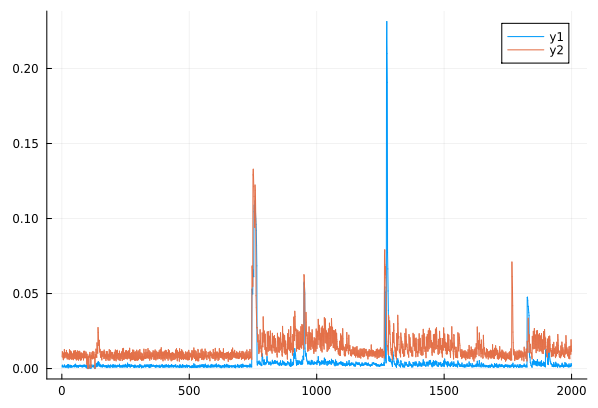
\includegraphics[scale=0.3]{h_and_v_one_byte}
			\caption{Mutual information for the horizontal value in orange and the vertical value in blue}
			\label{hvval}
		\end{figure}
		
		\subsection{Working CPA attack with another attack path}
		Let's note that there is a working simple CPA attack, as proven by Daemen et al. in \cite{cpa_lin} that we were able to reproduce as shown in the graphs \ref{graphs}. The idea is to first put the trigger before the linear-diffusion layer, then have for key hypothesis the three bits of the key which are xored to have the output $S_0^0$, and simplifying equations thanks to their observations.
		
		\begin{figure}[h]
			\centering
			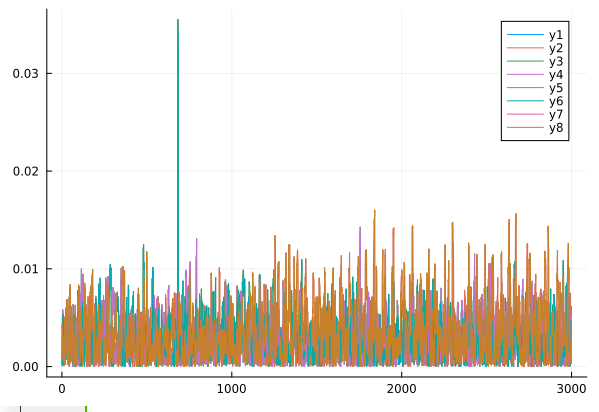
\includegraphics[scale=0.3]{graph_daemen}
			\caption{Absolute Pearson correlation between the output of $S_0^0$ and the power consumption as a function of time for each hypothesis for $(k_0,k_{36},k_{45})$}
			\label{graphs}
		\end{figure}
		
		This correlation allows to see a key providing a clear better correlation than any other: this is the right key, and in the same time the point of interest is shown clearly.\\
		We were able to reproduce the experiment and recover the entire key.
		
		
		\section{Using equations binding the input and output of the S-box}
		\subsection{Description of the equation} \label{sec_equ}
		Sarry \cite{these} describes in his thesis equations linking the output of the S-box to the value of the key, depending on the value of the nonce and of the IV \ref{link_k_s4}. These equations are described in the annex \ref{equations}.
		
		\begin{figure}[h]
			\centering
			\begin{tabular}{|c|c|}
				\hline
				$(n_0^j,n_1^j,IV^j)$&$S_4^j$\\
				\hline\hline
				$(0,0,0)$&$k_0^j$\\
				\hline
				$(0,0,1)$&$0$\\
				\hline
				$(0,1,0)$&$1$\\
				\hline
				$(0,1,1)$&$1 \oplus k_0^j$\\
				\hline
				$(1,0,0)$&$1 \oplus k_0^j$\\
				\hline
				$(1,0,1)$&$1$\\
				\hline
				$(1,1,0)$&$0$\\
				\hline
				$(1,1,1)$&$k_0^j$\\
				\hline
			\end{tabular}
			\caption{Link between $k_0^j$ and $S_4^j$ depending on $IV$ and $N$}
			\label{link_k_s4}
		\end{figure}
		
		\subsection{Attack path}
		According to \cite{cpa_analysis}, attacking the S-box by distinguishing key hypothesis is very difficult and needs numerous traces, as there are multiple keys that give strong correlations to their vertical Hamming Weight. We reproducted the experiment on 40K traces from the ChipWhisperer and were still unable to recover the key as multiple false key bit hypothesis gave good results.
		
		The goal is to use the equations described in the previous section \ref{sec_equ} to recover the key thanks to the value of $S_4$. So the problem is reduced to directly finding the output of the S-box in certain conditions (i.e. convenient values of nonces that is chosen by the attacker when asking for decryption). 
		
		Therefore, an other idea would be to directly have hypothesis for the output of the S-box, and to later find the associated key thanks to table \ref{link_k_s4}. To have thesse traces the attacker will ask the device to decrypt random ciphertexts and random tags 10K times, with a fixed convenient nonce and no matter the failure to authenticate, the algorithm will go through the attacked permutation from the initialization process.
		
		Let's formalize our attack: there will be 64 attacks for each column $j$ of the state where the target $t_j$ is $S-box(S_0^j||S_1^j||S_2^j \oplus \verb|const|_{16-a}^j||S_3^j||S_4^j)$, the vertical output of the S-box. Since $N$ is fixed and chosen, each execution of the decryption algorithm will output the same value $t_j$ after the first S-box of the initialization process. The attack path links this value to the measured power consumption. The theoritical attack path chosen in \ref{choice} is the Hamming weight of the target $t_j$ and the distinguisher the maximum of mutual information.
		
		Once an output $t_j$ is found, the bit $t_j^4$ is used to deduce $k_0^j$ and this algorithm entirely recovers $k_0$. Once that is done, $k_1$ is recovered using the equations \ref{k_1}, where $S_3^j$ has already been found as $t_j^3$.
		
		\begin{gather*} \label{k_1}
			S_3^j = (IV^j \oplus 1) \times (n_1^j \oplus n_0^j) \oplus IV^j \oplus k_0^j \oplus k_1^j\\
			k_1^j = (IV^j \oplus 1) \times (n_1^j \oplus n_0^j) \oplus IV^j \oplus k_0^j \oplus S_3^j\\
		\end{gather*}
		
		\subsection{Results}
		
		\section{Conclusion}
		
		\appendix
		
		\bibliographystyle{is-unsrt} 
		\bibliography{refs}
		
		\section{Notations} \label{notations}
		\begin{tabular}{ll}
				\hline
				\textbf{Notation}&\textbf{Definition}\\
				\hline
				$K$&Secret key\\
				$k_0$,$k_1$&first and last 64 bits of $K$\\
				$N$&Public nonce (i.e. changes at each\\
				&encryption)\\
				$n_0$,$n_1$&first and last 64 bits of $N$\\
				$S$&320-bit state\\
				IV&Initialization vector, 64-bit constant\\
				&of value \verb|0x00001000808c0001|\\
				$p$&The permutation for Ascon defined as \\
				&$p=p_L \circ p_S \circ p_C$, defined in section \ref{perm}\\
				S-box&Non-linear permutation function\\
				\verb|const|&Table of constants for $p_C$, see \ref{consts}\\
				\hline
				$x||y$&Concatenation of bitstrings $x$ and $y$\\
				$x>>>k$&Circular shift to the right of the word\\
				&$x$ by k bits\\
				$\oplus$&Bitwise xor\\
				\hline
				$S_i, \forall i \in \llbracket 0;4 \rrbracket$&$i^{th}$ 64-bit word of the 320-bit state $s$\\
				$w^j$&$j^{th}$ bit of the word $w$ (e.g. $S_i^j$) \\
				$p^k$&$\underbrace{p \circ p \circ ... \circ p}_{k times}$\\
				$0^k$&Concatenation of k bits 0 ($\underbrace{0||0|| ... |0}_{k times}$)\\
				$S_{<=k}$&For the bits numbered from 1 to 320\\ &bits from $S$ numbered from 1 to k\\
				$S_{>k}$&Bits of $S$ from k+1 to 320\\
				\hline
			\end{tabular}
			
		
		\section{Permutation layers} \label{perm}
		
		\subsection{Constant-addition layer $p_C$}
		If the permutation is applied $a$ times, the constant for the round $i$ is \verb|const|$_{16-a+i}$ in table \ref{consts}.\\
		If it is applied $b$ times, then \verb|const|$_{16-b+i}$ 
		
		\begin{figure}[h]
			\centering
			\footnotesize
			\begin{tabularx}{0.5\textwidth}{cc||cc}
				\hline
				$i$&\verb|const|$_i$&$i$&\verb|const|$_i$\\
				\hline
				0&\verb|0x000000000000003c|&8&\verb|0x00000000000000b4|\\
				1&\verb|0x000000000000002d|&9&\verb|0x00000000000000a5|\\
				2&\verb|0x000000000000001e|&10&\verb|0x0000000000000096|\\
				3&\verb|0x000000000000000f|&11&\verb|0x0000000000000087|\\
				4&\verb|0x00000000000000f0|&12&\verb|0x0000000000000078|\\
				5&\verb|0x00000000000000e1|&13&\verb|0x0000000000000069|\\
				6&\verb|0x00000000000000d2|&14&\verb|0x000000000000005a|\\
				7&\verb|0x00000000000000c1|&15&\verb|0x000000000000004b|\\
				\hline
			\end{tabularx}
			\caption{Constant-addition layer, each box representing a byte of one of the 64-bit words{}}
			\label{consts}
		\end{figure} 	
		
		\begin{figure}[h]
			\centering
			\begin{tabularx}{0.4\textwidth}{|*{8}{>{\centering\arraybackslash}X|}>{\centering\arraybackslash}X}
				\cline{1-8}
				&&&&&&&&$S_0$\\
				\cline{1-8}
				&&&&&&&&$S_1$\\
				\cline{1-8}
				&&&&&&& \LARGE $\oplus$&$S_2$\\
				\cline{1-8}
				&&&&&&&&$S_3$\\
				\cline{1-8}
				&&&&&&&&$S_4$\\
				\cline{1-8}
			\end{tabularx}
			\caption{Constant-addition layer, each box representing a byte of one of the 64-bit words{}}
		\end{figure} 	

		\subsection{Substitution layer $p_S$}
		Let's write $\Sigma=p_S(S)$\\
		The substitution layer computes for each $i \in \llbracket 1;64 \rrbracket$:
			$$(\Sigma_0^j,\Sigma_1^j,\Sigma_2^j,\Sigma_3^j,\Sigma_4^j) = S-box(S_0^j||S_1^j||S_2^j||S_3^j||S_4^j),$$
			
		with the S-box the lookup table \ref{lookup_sbox}.
		
		\begin{figure}[h]
			\small
			\centering
			\begin{tabular}{|c||*{8}{c|}}
				\hline
				$x$&0&1&2&3&4&5&6&7\\
				\hline
				$S-box(x)$&4&b&1f&14&1a&15&9&2\\
				\hline\hline
				$x$&8&9&a&b&c&d&e&f\\
				\hline
				$S-box(x)$&1b&5&8&12&1d&3&6&1c\\
				\hline\hline
				$x$&10&11&12&13&14&15&16&17\\
				\hline
				$S-box(x)$&1e&13&7&e&0&d&11&18\\
				\hline\hline
				$x$&18&19&1a&1b&1c&1d&1e&1f\\
				\hline
				$S-box(x)$&10&c&1&19&16&a&f&17\\
				\hline
			\end{tabular}
			\caption{Lookup table for the 5-bit S-box}
			\label{lookup_sbox}
		\end{figure}
		
		It can also be computed using the circuit \ref{circuit_sbox}, which gives the equations \ref{equations_sbox}.
		
		\begin{figure}[H]
			\centering
			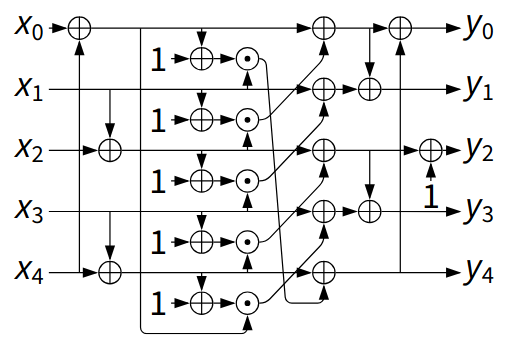
\includegraphics[scale=0.4]{circuit}
			\caption{Equivalent circuit to compute the S-box, from \cite{norme}}
			\label{circuit_sbox}
		\end{figure}
		
		\begin{figure}[H]
			\centering
			\begin{lstlisting}[style=CStyle]
			state[0] ^= state[4];
			state[4] ^= state[3];
			state[2] ^= state[1];
			uint64_t t0 = ~state[0];
			uint64_t t1 = ~state[1];
			uint64_t t2 = ~state[2];
			uint64_t t3 = ~state[3];
			uint64_t t4 = ~state[4];
			t0 &= state[1];
			t1 &= state[2];
			t2 &= state[3];
			t3 &= state[4];
			t4 &= state[0];
			state[0] ^= t1
			; state[1] ^= t2;
			state[2] ^= t3;
			state[3] ^= t4;
			state[4] ^= t0;
			state[1] ^= state[0];
			state[0] ^= state[4];
			state[3] ^= state[2];
			state[2] =~ state[2];
			\end{lstlisting}
			\caption{Equations to compute the S-box}
			\label{equations_sbox}
		\end{figure}
		
		\subsection{Linear-diffusion layer $p_L$}
		It provides diffusion throughout each word $S_i \leftarrow \Sigma_i(S_i)$:
		
		\begin{gather*}
			\Sigma_0(S_0) = S_0 \oplus (S_0 >>> 19) \oplus (S_0 >>> 28)\\
			\Sigma_1(S_1) = S_1 \oplus (S_1 >>> 61) \oplus (S_1 >>> 39)\\
			\Sigma_2(S_2) = S_2 \oplus (S_2 >>> \;  1) \oplus (S_2 >>> \; 6)\\
			\Sigma_3(S_3) = S_3 \oplus (S_3 >>> 10) \oplus (S_3 >>> 17)\\
			\Sigma_4(S_4) = S_4 \oplus (S_4 >>> \; 7) \oplus (S_4 >>> 41)\\
		\end{gather*}
		
		\section{Equations for linking the output of the S-box to the key} \label{equations}
		\begin{gather*}
			S_4^j = n_o^j \oplus n_1^j \oplus k_0^j \times (1 \oplus IV^j \oplus n_1^j)\\
			S _4^j =\left \{	
				\begin{array}{ll}
					k_0^j \times (1 \oplus IV^j) & if\ (n_0^j,n_1^j)=(0,0)\\
					k_0^j \times IV^j & if\ (n_0^j,n_1^j)=(1,1)\\
					1 \oplus k_0^j \times IV^j & if\ (n_0^j,n_1^j)=(0,1)\\
					1 \oplus k_0^j \times (1 \oplus IV^j) & if\ (n_0^j,n_1^j)=(1,0)\\
				\end{array}
					\right.
		\end{gather*}
		 
		 \noindent Then if $IV^j = 0$: 
		 $$S _4^j =\left \{	
		 \begin{array}{ll}
		 	k_0^j& if\ (n_0^j,n_1^j)=(0,0)\\
		 	0& if\ (n_0^j,n_1^j)=(1,1)\\
		 	1& if\ (n_0^j,n_1^j)=(0,1)\\
		 	1 \oplus k_0^j& if\ (n_0^j,n_1^j)=(1,0)\\
		 \end{array}
		 \right.$$
		 
		 \noindent Otherwise, if $IV^j = 1$:
		 $$S _4^j =\left \{	
		 \begin{array}{ll}
		 	0& if\ (n_0^j,n_1^j)=(0,0)\\
		 	k_0^j& if\ (n_0^j,n_1^j)=(1,1)\\
		 	1 \oplus k_0^j& if\ (n_0^j,n_1^j)=(0,1)\\
		 	1& if\ (n_0^j,n_1^j)=(1,0)\\
		 \end{array}
		 \right.$$

	\end{document}
	